%\begin{figure}[h]
%    \centering
%    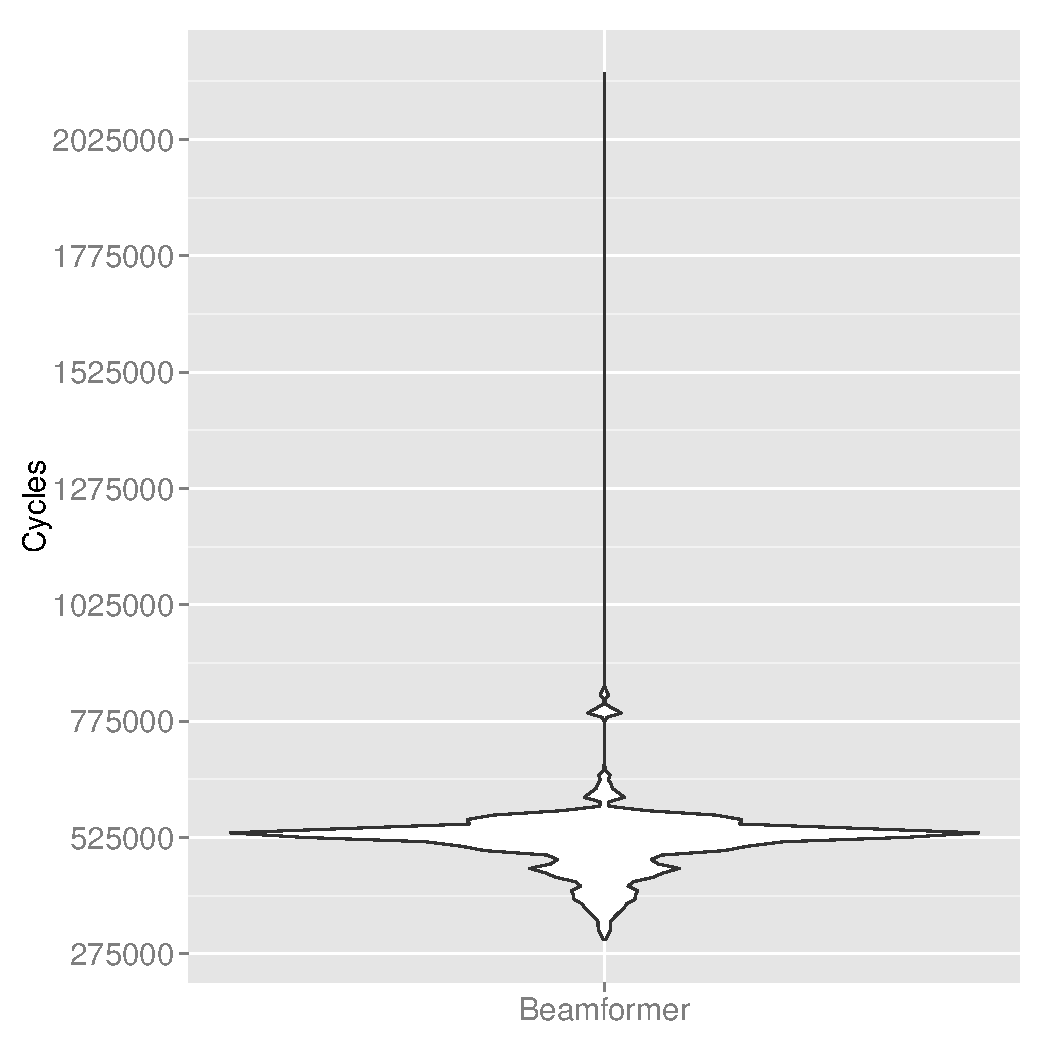
\includegraphics[width=0.7\textwidth]{streamit-paper/graphics/beamformer_motivation.pdf}
%    \caption{Distribution of the runtime for Beamformer resulting from an exhaustively exploration of the hardware/software co-design space.
%     The application has been partitioned into different number of threads and core compositions.}
%     \label{fig:beamformermotiv}
%\end{figure}
\subsection{Finding an optimal configuration}
This section motivates the difficulty of finding a good combination of thread and core partitioning.
First, a simple experiment is conducted where the \bench{FilterBank} StreamIt benchmark is analysed using a 16 core dynamic multicore processor.
%Maybe reform this sentence
\bench{FilterBank} distributes its inputs amongst an array of discrete fourier transform (DFT) filters, the outputs of the DFT filters are down-sampled, up-sampled and then recombined to form a processed signal~\cite{streamitrepo}.
The program's tasks are partitioned into threads and a various number of cores are allocated to each of the threads.
Since one of the threads is the master which creates and joins all worker threads, this means that the application can be partitioned in up to 15 threads, and 15 cores can be used for those threads.
As each thread must have at least one core assigned to it, and not all cores have to be grouped together, the total number of configurations are:

\begin{equation}
15 + \sum_{threads=2}^{15} \bigg( \sum_{cores=threads}^{15} \frac{(cores-1)!}{(threads-1)!((cores-1)-(threads-1))!}\bigg)
\label{eq:comb}
\end{equation}

In Equation~\ref{eq:comb}, the constant 15 represents the 15 different number of cores that can be composed for the single threaded version.
There are 32,767 combinations (exhaustive space) of thread mappings and core compositions pairings that can be generated.
In this chapter, a design point represents one of these 32,767 different configurations.

\begin{figure}[t]
    \centering
    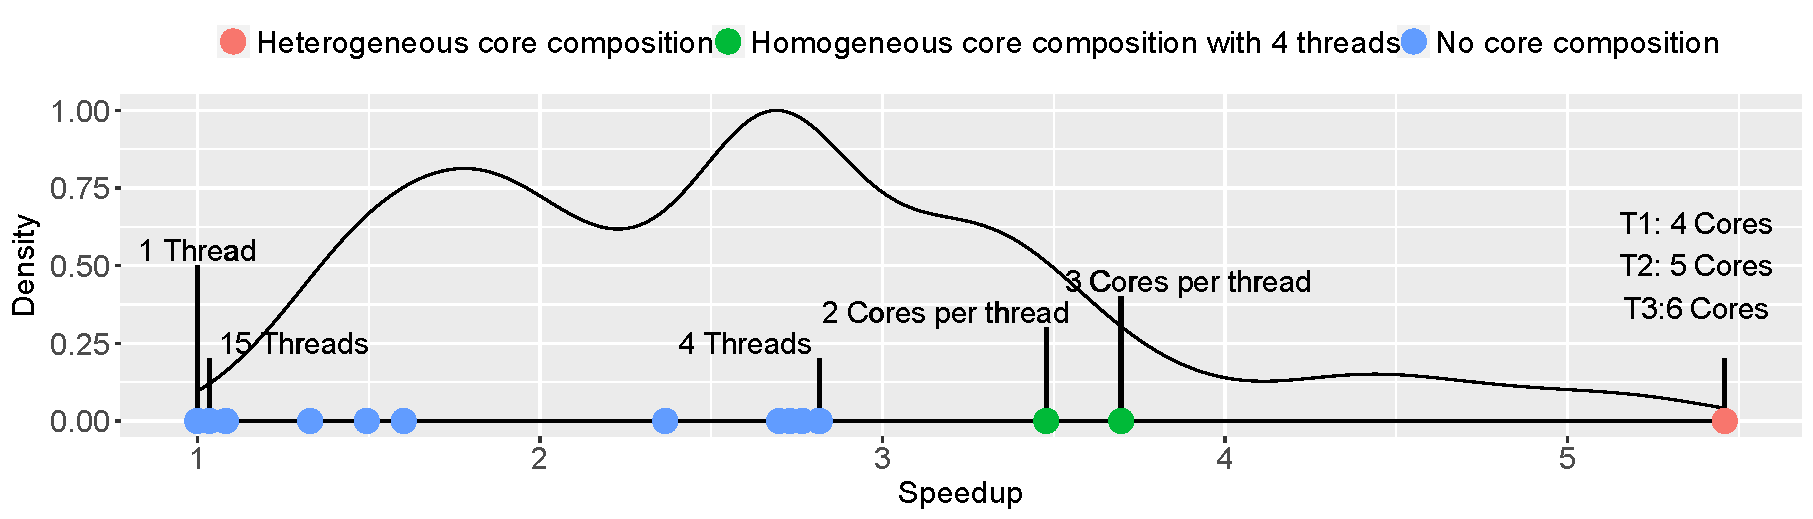
\includegraphics[width=1\textwidth]{streamit-paper/graphics/filterbank_motivation_4.pdf}
    \caption{Distribution of speedups for FilterBank when using different core composition and thread pairings compared to single-core single thread. The dots on the X-axis represent specific configurations.}
     \label{fig:threadcoremotiv}
	 \vspace{-1em}
\end{figure}

Figure~\ref{fig:threadcoremotiv} presents the speedup distribution from a subset of the co-design space of \bench{FilterBank} as a density graph.
The speedup is measured by comparing the performance of the design point to that of a single-core/single thread.
A single-core/single thread is used here as it represents the default "unmodified" configuration.
For this experiment, 1316 different thread/core combinations are explored; the reason this number is chosen is explained later on in section~\ref{chp:stream:sec:setup}.

As can be seen in figure~\ref{fig:threadcoremotiv}, the majority of the design points result in a speedup of 2.7x.
The best speedups however are far fewer than the average case (4x smaller density) and can improve performance by up to almost 6x.
Thus, if a good configuration is found, this can yield an important speedup compared to the average configuration.
However since the number of good configurations is low, this underlines the notion that finding a combination of threads and cores is a non-trivial endeavor, as randomly choosing a configuration will result in a sub-optimal performance.
Indeed, even if the average case is 2.7x faster than a single core, Figure~\ref{fig:threadcoremotiv} shows that there exists a good number of configurations that can lead to less than average speedups.

\subsection{Minimizing the search space}
Whilst there exists a large variety of thread-core combinations, certain design choices can be used to try and minimise the space.
For example, choosing to only do multithreading reduces the search space to 15 possible solutions whilst only combinations that lead to homogeneous core compositions reduces the search space to:

\begin{equation}
\sum_{threads=1}^{15} \lfloor\frac{15}{threads}\rfloor= 45
\end{equation}

where the constant 15 represents the number of cores available.
Using only homogeneous core compositions, which facilitates the core partitioning decision, would therefore lead to 45 possible solutions.
However, reducing the search space limits the potential obtainable speedup.
Figure~\ref{fig:threadcoremotiv} shows the performance distribution of these specific design points.
Their location on the X-axis represents the speedup obtained for that specific configuration.
The points represent a set of different design choices such as only using multithreading, using homogeneous core-compositions with threads and using heterogeneous core-compositions with threads.

Using only multithreading can lead to some performance improvements, however it will not result in the optimal performance.
For the \bench{FilterBank} benchmark, 4 threads leads to the fastest execution time when only using multithreading.
This performance is in the highest peak of the density curve, which means that finding the best number of threads for the benchmark will only lead to average performance improvements in this case.
However, using too many threads, such as 15 threads, leads to a degraded performance compared to the average.
This is due to the fact that the communication overhead between threads will be too high.

To explore homogeneous core composition, the optimal number of threads, which is the number of threads that leads to the fastest execution time without core-composition is used as a baseline.
In this case only 2 homogeneous pairings exist: 2 cores fused for each of the 4 threads or 3 cores fused for each of the 4 threads.
Figure~\ref{fig:threadcoremotiv} shows that homogeneous core-composition will outperform only using multithreading by 1.3x, however it is not the optimal solution.
In the end, using a heterogeneous configuration leads to a 1.5x speedup compared to the fastest homogeneous configuration.
Therefore, it is important to consider all possible configurations to ensure the possibility of obtaining the best performance.

\subsection{Summary}
This section shows that multi-threading with heterogeneous core-composition is the optimal solution.
This means that the total space must be explored in order to ensure that the best speedup can be found.
Due to the size of the space and the fact that there can be no apriori about good configurations, using machine learning to predict configurations is a promising approach. % be used to predict good configurations.
By exploring a set of StreamIt benchmarks a machine learning model can learn what features correlate with the correct configuration.
This example illustrates the necessity for designing the technique to predict both the optimal number of threads and core composition to use.
The next section will present a more in-depth analysis of the design space before presenting our machine-learning predictive model.
